\section{Locality of Reuse}
\label{sec:locality}

This section answers Q1 on the oracle-admitted calls of the potential tier. For every call whose replay is
equivalent to the recorded observation, it locates the first earlier exact repeat.

\subsection{Cross-Attempt Locality}
\label{sec:scope}

Figure~\ref{fig:scope} decomposes the 70,173 oracle-admitted calls by the innermost scope of an earlier exact repeat.
Repeats from other attempts of the same task and model carry 37.3\% of the calls. They carry 33.5\% of the isolated DB-execution time and 60.8\% of the payload bytes. Repeats within the same session carry 6.0\%, 9.3\% and 13.7\%.
Repeats seen only in another model's or another task's runs add 4.0\%, 2.3\% and 6.1\%. Cross-attempt repeats are
skewed toward large results, since they carry 60.8\% of the bytes and 33.5\% of the time. The files that hold large
results are therefore the main target for a cache (Section~\ref{sec:ownership}).

The per-task picture is sharper than the pooled one. The median task attributes 41.2\% of its DB time to
cross-attempt repeats (95\% CI 36.1--49.3\%) and 3.2\% to repeats within a session (2.2--4.6\%). For bytes the
medians are 46.4\% and 3.5\%. The paired difference is significant over the 54 tasks (Wilcoxon, Holm-corrected
$p=2.6\times10^{-9}$, rank-biserial $r=0.997$). It survives the nesting of tasks in datasets. A bootstrap that
resamples whole datasets gives 41.2\% (34.6--50.2\%) against 3.2\% (1.8--6.5\%). The cross-attempt median exceeds the
session median in all 12 datasets (Table~\ref{tab:datasets}, sign test $p=0.0005$). Task by task
(Figure~\ref{fig:pertask}), the cross-attempt share of DB time exceeds the session share in 53 of the 54 tasks. It is
at least three times as large in 51. For bytes the counts are 52 and 43.

\subsection{Scaling with the Number of Attempts}
\label{sec:growth}

Cross-attempt locality turns into savings that grow with the number of attempts. Figure~\ref{fig:ncurve} shows an
unbounded, oracle-gated simulation. A cache shared by the batch (S2) saves 9.6\%, 16.6\%, 24.1\%, 32.2\% and 47.0\%
of the isolated DB-execution time at $N=2$, 4, 8, 16 and 50. These values are medians over tasks on the
oracle-admitted calls. A session cache (S1) stays between 3.0\% and 3.4\% at every $N$. The median task reaches a
20\% saving at $N=8$, where 64.8\% of tasks reach it. At $N=4$, 35.2\% of tasks already save at least 20\% and
79.6\% at least 10\%. The per-task ratio of S2 to S1 DB time falls from 0.943 at $N=2$ to 0.801 at $N=8$. The Holm-corrected $p$ is $4.6\times10^{-9}$ at $N=2$, 4 and 8. Payload bytes follow the same curve, with 23.9\% saved at
$N=8$. Resampling whole datasets widens the $N=8$ interval to 18.4--30.3\% without moving the median. The saving does
not depend on which of the three replays supplies a query's time. At $N=8$ it is 24.1\% (task-bootstrap 95\% CI
21.1--28.8\%) with the median of the completed executions. It is 23.3\% (20.9--28.1\%) with the first execution and
24.1\% (21.1--28.9\%) with the steady-state ones.

\subsection{Heterogeneity and Robustness}
\label{sec:robust}

% Fig. 2 -- locality per task and under different conditions (figure*, Section 4)
\begin{figure*}[tbp]
  \centering
  \subcaptionbox{Per task: session share against cross-attempt share\label{fig:pertask}}{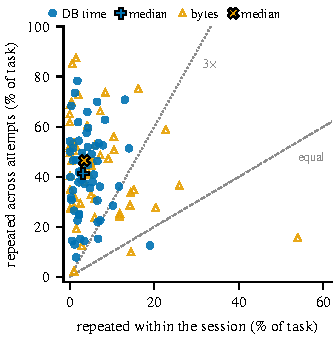
\includegraphics[height=2.05in]{figures/fig2a_pertask}}\hfill
  \subcaptionbox{Pooled share of isolated DB-execution time under different conditions\label{fig:conditions}}{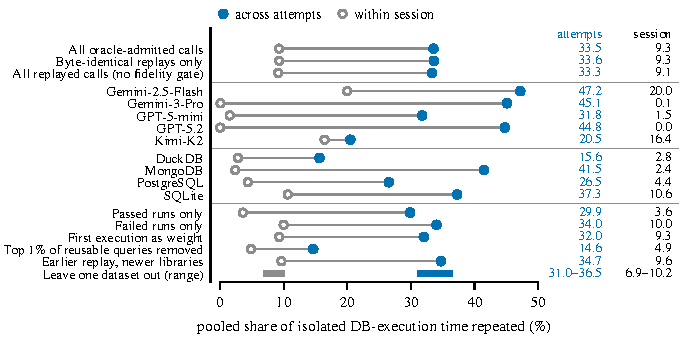
\includegraphics[height=2.05in]{figures/fig2b_conditions}}
  \caption{Locality per task and under different conditions. (a) One point per task and weight for the 54 tasks, on the oracle-admitted calls. Circles show isolated
  DB-execution time and triangles payload bytes. The axes give the share repeated within the session ($x$) and
  across attempts of the same task and model ($y$). The dashed line is $y=x$, the dotted line is
  $y=3x$, and large markers are task medians. (b) Pooled DB-time shares on the 70,173 oracle-admitted calls, a named
  subset, or another population. Byte-identical replays cover 66,556 calls, all replayed calls 76,141, and the earlier
  replay its 62,419 byte-identical calls. Shares are means over 200 random attempt orders, with 20 orders for the two
  gate variants and 50 for the top-1\% removal.}
  \label{fig:locality}
  \Description{Two panels. Left: a scatter plot with two points per task, one for DB time and one for bytes. Nearly all lie above the equal-share line and most above the three-times line. Right: one row per condition. The cross-attempt estimate lies to the right of the within-session estimate in every row, with the leave-one-dataset-out row shown as ranges.}
\end{figure*}


Every model repeats more across attempts than within its session, by different margins
(Figure~\ref{fig:conditions}). GPT-5.2 and Gemini-3-Pro almost never re-issue a query inside a session and repeat
44.8\% and 45.1\% of their DB time across attempts. Gemini-2.5-Flash and Kimi-K2 also repeat inside their sessions
(20.0\% and 16.4\%). At $N=4$ the median task--model saving ranges from 9.0\% for GPT-5-mini to 23.5\% for
Gemini-2.5-Flash.

The ordering persists across engines, fidelity gates, run outcomes, time weights, query removal, dataset removal and
an earlier replay (Figure~\ref{fig:conditions}). Reusable time is concentrated: 67 of the 6,641 reusable queries
(1\%) hold 68.7\% of it. Removing those queries lowers the pooled cross-attempt share to 14.6\%. The per-task medians
barely move (39.3\% against 2.6\%), and the median $N=8$ saving stays at 22.3\%. The earlier replay used newer
library versions (DuckDB 1.5.6, pandas 3.0.6), no pinned time zone and a less strict check of the database load.

The CIDR'26 vision reports that distinct sub-plans are a small fraction of those generated over many attempts
\cite{liu2026overlords}. We reproduce that statistic on DAB's DuckDB-native calls (179 task--model cells, 27,388
calls). The median share of distinct sub-plans per cell is 21.7\% for single operators. It rises to 77.8\% for
sub-plans of six or more operators, while 54.8\% of whole query texts are distinct. For reusing complete results, whole-query repetition across attempts is what a system can exploit.

\subsection{Generalization across Agent Harnesses}
\label{sec:xharness}

% Table 4 -- cross-harness (column width)
\begin{table}[htbp]
  \caption{Exact-call repetition in four public leaderboard harnesses on DAB's tasks and in the first five runs of the
  released DAB traces. The analysis is at trace level, without replay, on the exact database and query text. Qwen3.8
  denotes Qwen3.8-Flash-Next, and DeepSeek-v4.1 denotes DeepSeek-v4.1-flash. Session and other-attempt columns are
  pooled call shares averaged over 50 random attempt orders. $N{=}5$ is the median share of calls that repeat an
  earlier call among five attempts (50 resamples), over the listed number of tasks with five available runs.}
  \label{tab:xharness}
  \footnotesize\setlength{\tabcolsep}{2.5pt}
  \begin{tabular}{@{}lrrrrr@{}}
\toprule
Harness / model & Runs & Calls & \% session & \% other att. & $N{=}5$ \% (tasks) \\
\midrule
Phoenix-CLI / Opus 5 & 270 & 2,937 & 1.7 & 13.4 & 15.5 (54) \\
DAB scaffold / Qwen3.8 & 270 & 3,294 & 0.1 & 15.9 & 17.9 (54) \\
Scout / GLM-5.2 & 249 & 1,490 & 0.3 & 5.7 & 7.8 (37) \\
Stela / DeepSeek-v4.1 & 264 & 3,306 & 0.2 & 5.0 & 4.9 (48) \\
\midrule
DAB / Gemini-2.5-Flash & 269 & 958 & 18.7 & 14.7 & 30.0 (53) \\
DAB / Gemini-3-Pro & 270 & 1,708 & 0.1 & 23.2 & 24.6 (54) \\
DAB / GPT-5-mini & 270 & 1,388 & 0.5 & 8.6 & 11.2 (54) \\
DAB / GPT-5.2 & 270 & 1,093 & 0.1 & 13.5 & 13.2 (54) \\
DAB / Kimi-K2 & 266 & 2,287 & 11.6 & 8.3 & 13.3 (51) \\
\bottomrule
\end{tabular}

\end{table}


The locality does not stem from DAB's own scaffold. We extracted every database call from the public trace archives
of four leaderboard submissions. They ran DAB's tasks with other agent harnesses and models, up to five trials per
task (Table~\ref{tab:xharness}). In all four, exact repeats across attempts outnumber repeats within a session. The
call shares are 13.4\% against 1.7\% for Phoenix-CLI and 15.9\% against 0.1\% for DAB's scaffold with Qwen3.8. They
are 5.7\% against 0.3\% for Scout and 5.0\% against 0.2\% for Stela. At five attempts the median task repeats
4.9--17.9\% of its calls. We also replay these queries with DAB's tool semantics in the pinned runtime, without a
fidelity comparison with the result the harness recorded. Exact repeats across attempts then account for 6.9\%
against 4.8\% of the replay-stable DB time for Phoenix-CLI. The shares are 12.3\% against 0.0\% for Qwen3.8, 9.4\%
against 0.05\% for Scout and 4.0\% against 0.03\% for Stela. The byte ordering holds for Qwen3.8, Scout and Stela.
For Phoenix-CLI, repeats across attempts and within the session account for 0.2\% and 3.4\% of the replay-stable
bytes. At five attempts, the median-task saving is 13.1\%, 14.4\%, 2.9\% and 2.4\% of the replay-stable DB time.
These medians cover 54, 54, 37 and 48 tasks with five runs that contain database calls. 
The Phoenix-CLI traces carry timestamps, and the median LLM turn between a tool result and the next call takes
5.2\,s. Attempts that run concurrently therefore overlap on their queries, the setting of
Section~\ref{sec:concurrency}.
